\documentclass[aspectratio=169]{beamer}
\usepackage{generic}
\newcommand\arrow{~$\rightarrow$~~}
\begin{document}

\begin{frame}
  \title{\vspace{-4ex}
    Open and Reproducible Fisheries Science\\[0.5ex]
    \Large\it Standardized workflows at ICES and FAO}
  \author{\vspace{-16ex}\small\darkgreen
    {\bf Arni Magnusson$^1$, Colin Millar$^2$, Rishi Sharma$^3$}\\[1ex]
    \scriptsize\darkgray
    $^1$ Pacific Community (SPC), Nouméa, New Caledonia\\
    $^2$ International Council for the Exploration of the Sea (ICES),
    Copenhagen, Denmark\\
    $^3$ UN Food and Agriculture Organization (FAO), Rome, Italy}
  \date{
    CAPAM Good Practices Workshop\\[0.5ex]
    Rome, 24 Oct 2022}
  \titlepage
\end{frame}

% ______________________________________________________________________________

\begin{frame}{Overview}
  \begin{itemize}
    \item[] {\bf\darkblue Why} \comment{repeatability, institutional memory,
      reviewability, scientific method,\\
      \h{8.5ex}interregional research, dissemination, collaboration,
      traceability, credibility}\\[3ex]
    \item[] {\bf\darkblue Open} \comment{scripts, data, software}\\[3ex]
    \item[] {\bf\darkblue Reproducible} \comment{standardized sequential R
      scripts, version control}\\[3ex]
    \item[] {\bf\darkblue Infrastructure}
    \comment{2021 UN Recommendation on Open Science, working group,\\
      \h{18.6ex}GitHub, TAF, data management, ICES, FAO, GFCM, SPC}\\[3ex]
    \item[] {\bf\darkblue Recommendations}
    \comment{relative paths, dependencies, 1st and 2nd class scripts,\\
      \h{23.9ex}complete workflow, data preparation, partially open}\\[3ex]
  \end{itemize}
\end{frame}

% ______________________________________________________________________________

\begin{frame}{Why open and reproducible}
  \begin{itemize}
    \item[] Peer reviewability and reproducibility are {\bf core
      principles}\\[0.2ex]
    underpinning the {\bf scientific method}\\[0.5ex]
    \arrow {\small Reproducibility distinguishes between arbitrary analyses and
      science}\\
    \arrow {\small Some assessments are more reviewable than others}\\[5ex]
    \item[] Easy to pick up a stock assessment from a previous year and\\[0.2ex]
    run an {\bf update assessment}\\[0.5ex]
    \arrow {\small Especially important when a new scientist is doing the
      assessment}\\[4ex]
  \end{itemize}
\end{frame}

% ______________________________________________________________________________

\begin{frame}{Why open and reproducible (cont)}
  \begin{itemize}
    \item[] Easy to modify model settings and rerun the {\bf entire
      workflow}\\[0.5ex]
    \arrow {\small Allows more thorough analyses, exploration,
      improvements}\\[5ex]
    \item[] {\bf Share data} that others can use\\[0.5ex]
    \arrow {\small Dissemination, machine and human readable}\\
    \arrow {\small Interregional research, collaboration}\\[5ex]
    \item[] {\bf Traceability}\\[0.5ex]
    \arrow {\small Credibility, buy-in}\\[4ex]
  \end{itemize}
\end{frame}

% ______________________________________________________________________________

\begin{frame}
  \begin{columns}[T]
    \column{0.16\textwidth}
    \column{0.8\textwidth}
    \vspace{-5ex}
    \begin{center}
      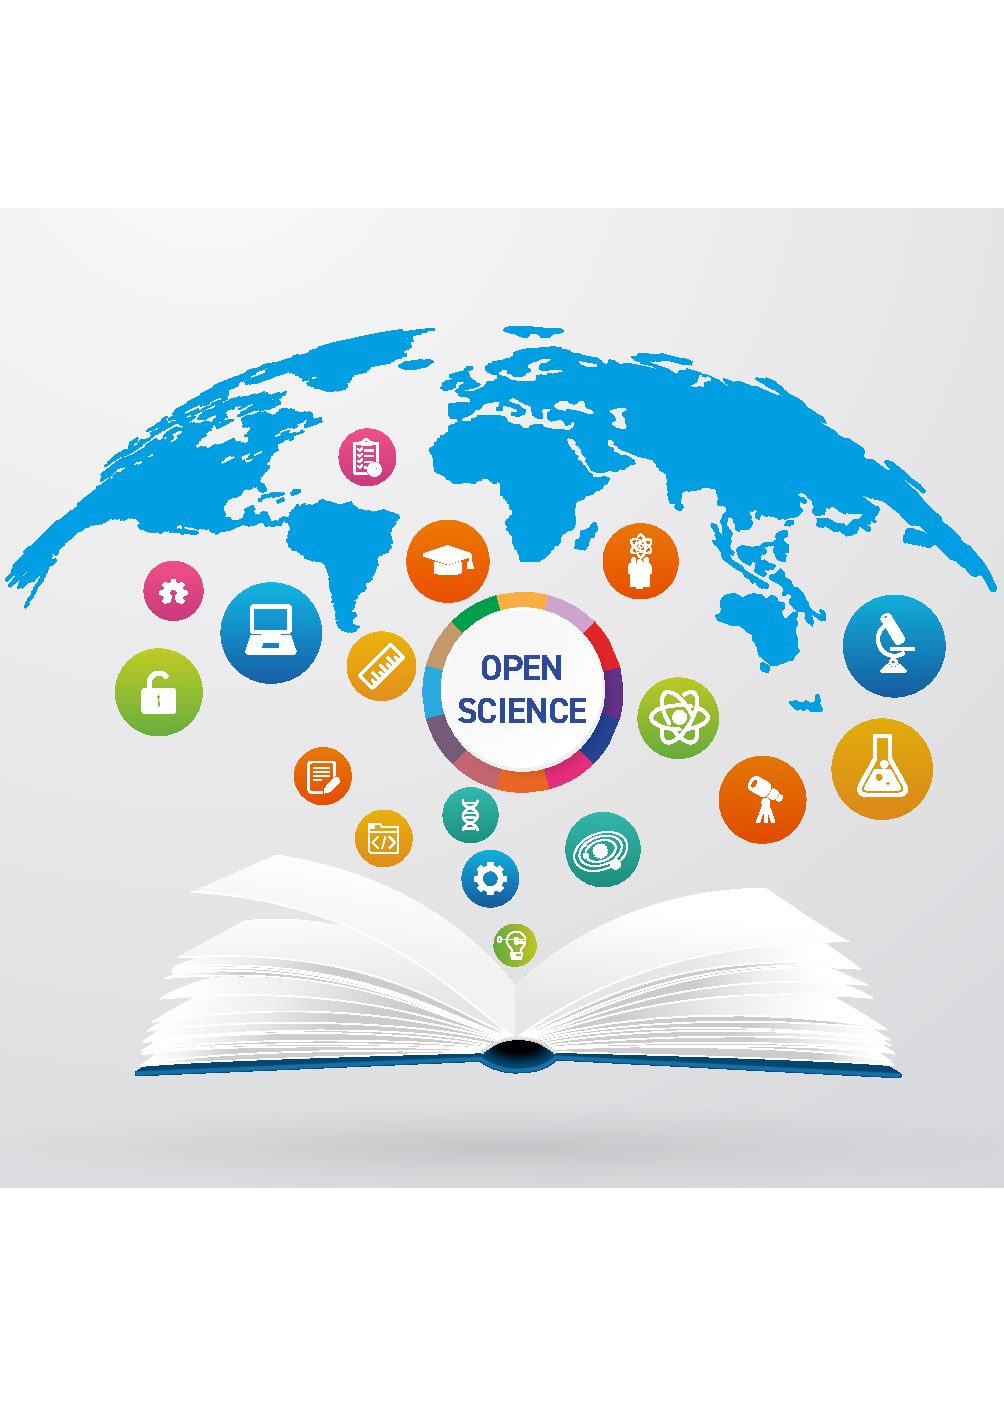
\includegraphics[height=1.05\textheight]{open_science}
    \end{center}
    \column{0.24\textwidth}
    \vspace{41ex}
    \tiny\gray
    \h{-2ex}Compare to 1990s:\\[1ex]
    litdb, photocopy\\[0.5ex]
    buying software\\[0.5ex]
    typing numbers
  \end{columns}
\end{frame}

% ______________________________________________________________________________

\begin{frame}{Open}
  \begin{description}
    \item[\bf Scripts~] GitHub\\[5ex]
    \item[\bf Data~] Static HTML\\[0.5ex]
    GitHub\\[0.55ex]
    Data warehouse\\[0.5ex]
    Web services\\[5ex]
    \item[\bf Software~] GitHub\\[0.5ex]
    Releases\\[3ex]
  \end{description}
\end{frame}

% ______________________________________________________________________________

\begin{frame}{How Open?}
  \begin{columns}[T]
    \column{0.24\textwidth}\darkgray
    ~Not provided online\\[1ex]
    ~Sensitive data
    \column{0.26\textwidth}\darkgreen
    Requires login\\[1ex]
    Available by request\\[1ex]
    Part private, part open\\[1ex]
    Hard to find
    \column{0.28\textwidth}\green
    Fully open\\[0.5ex]
    Easy to find and browse
  \end{columns}
\end{frame}

% ______________________________________________________________________________

\begin{frame}{Reproducible Analysis}\small
  \textbf{\darkgreen Can be run on any computer}\\[-0.6ex]
  \begin{itemize}
    \item[] By different people\\[-0.6ex]
    \item[] On different operating systems\\[-0.6ex]
    \item[] In different software environments\\[3ex]
  \end{itemize}
  \textbf{\darkgreen Can be run later}\\[-0.6ex]
  \begin{itemize}
    \item[] Next week\\[-0.6ex]
    \item[] Next year\\[-0.6ex]
    \item[] 5--10 years from now\\[3ex]
  \end{itemize}
  \textbf{\darkgreen Can be modified and rerun}\\[-0.6ex]
  \begin{itemize}
    \item[] With different data\\[-0.6ex]
    \item[] With different model settings
  \end{itemize}
\end{frame}

% ______________________________________________________________________________

\begin{frame}{How Reproducible?}\small
  A gradient from low $\rightarrow$ high {\bf quality of science}, in terms of
  reproducibility:\\
  \begin{enumerate}
    \item Here's the management advice -- trust me, I did the math\\[-0.5ex]
    \item I used the model published in this paper and here are the data
    tables and results\\[-0.5ex]
    \item I used these exact equations and preprocessed the data in this
    manner\\[-0.5ex]
    \item Here are some scripts that give the general idea\\[-0.5ex]
    \item Here are scripts that run on my computer, as a complete workflow
    without errors\\[-0.5ex]
    \item Here are scripts that should run on your computer, along with all
    input files and\\
    software dependencies\\[-0.5ex]
    \item I've cleaned up the directory to include only files required to run
    the core analysis,\\
    tested on another computer, with exact instructions on how to run\\[-0.5ex]
    \item Adopted a standard reproducible format for the analysis
  \end{enumerate}
\end{frame}

% ______________________________________________________________________________

\begin{frame}{How to Make an Analysis Reproducible}\small
  \begin{description}
    \item[\bf R scripts] Relative paths (data/catch.dat)\\
    Can be run from command line: {\tt Rscript myscript.R}\\
    Manageable size\\[3ex]
    \item[\bf General structure] 1. Load packages\\
    \h{5ex}2. Read files\\
    \h{5ex}3. Do the work\\
    \h{5ex}4. Write files\\[3ex]
    \item[\bf Standardize further] One script prepares data\\
    \h{7.1ex}Another script runs the core analysis\\
    \h{7.1ex}Third script gathers the results\\
    \h{7.1ex}Fourth script produces plots and formatted tables for report\\
    \h{7.1ex}$\Rightarrow$ Every script is self-contained, reading files from
    previous steps\\
    \h{7.1ex}$\Rightarrow$ Every analysis is structured the same, anyone can
    pick up and run
  \end{description}
  \vspace{2ex}
\end{frame}

% ______________________________________________________________________________

\begin{frame}{Transparent Assessment Framework (TAF)}
  Supports open and reproducible science\\[2.5ex]
  More than anything, an {\bf agreed way} to work with R scripts\\[2.5ex]
  Launched in 2018\\[2.5ex]
  Developed by ICES, used around the world\\[2.5ex]
  {\blue\href{https://taf.ices.dk}{taf.ices.dk}}\\[1ex]
\end{frame}

% ______________________________________________________________________________

\begin{frame}
  \centering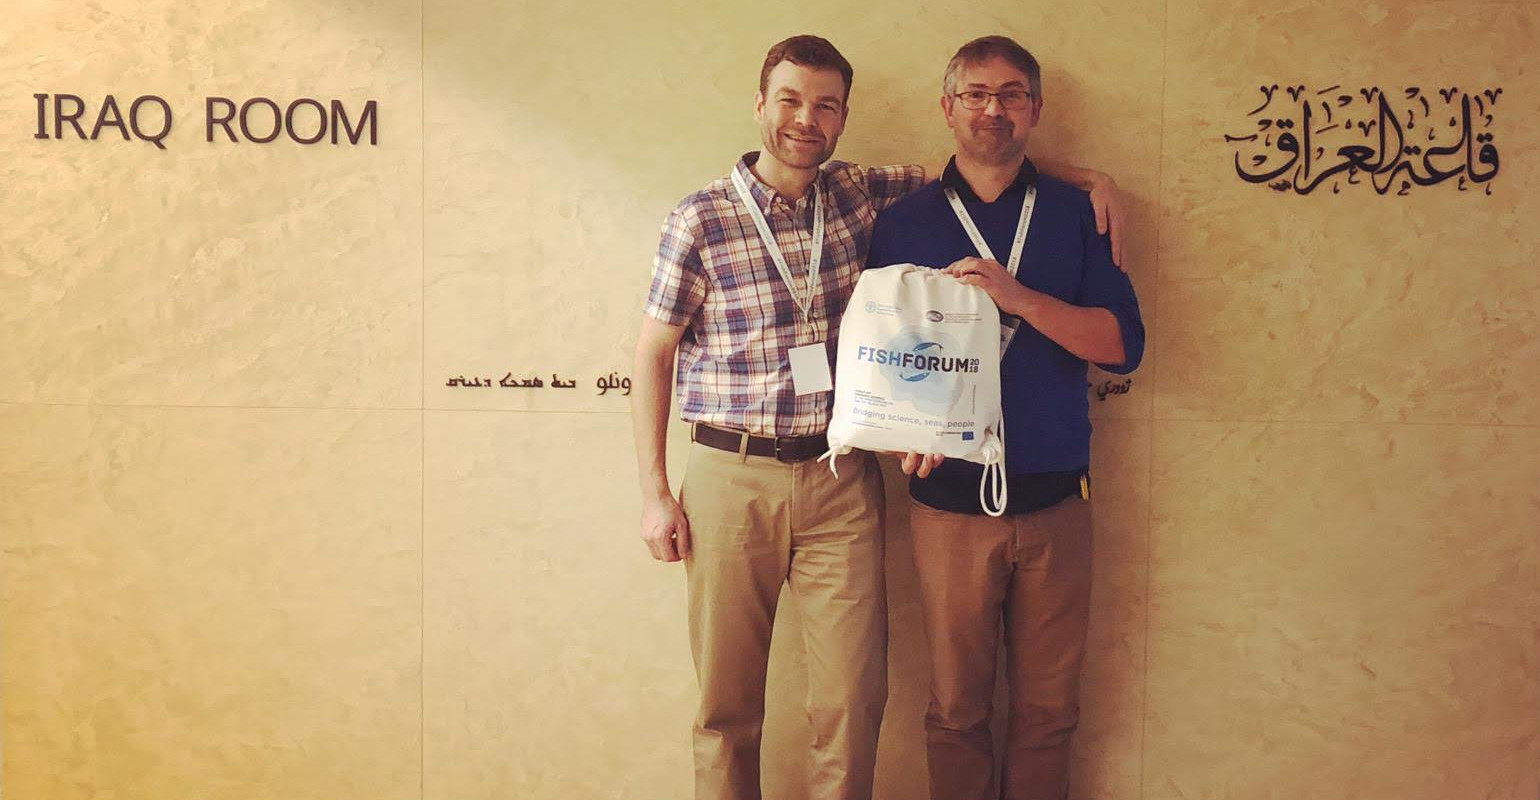
\includegraphics[width=\textwidth]{iraq_room}
\end{frame}

% ______________________________________________________________________________

\begin{frame}{Transparent Assessment Framework (TAF)}\small
  \textdarkgreen{\bf TAF applications}\\
  \begin{itemize}
    \item[] Around 30 ICES stock assessments each year\\[-0.5ex]
    \item[] ICES survey indices\\[-0.5ex]
    \item[] ICES catch at age\\[-0.5ex]
    \item[] ICES fisheries overviews\\[-0.5ex]
    \item[] FAO SOFIA -- under development
  \end{itemize}
  \vspace{2ex}
  {\darkgreen\bf R packages} TAF, icesTAF, SOFIA\\[4ex]
  {\darkgreen\bf Version control} ~--~ software and data\\[4ex]
  {\darkgreen\bf Data provenance} ~--~ who, what, where
  \vspace{4ex}
\end{frame}

% ______________________________________________________________________________

\begin{frame}{SOFIA-TAF}
  \begin{itemize}
    \item[] Standardized structure to organize the SOFIA analyses\\[3ex]
    \item[] All the fisheries in the world\\[3ex]
    \item[] Converted from monolithic R Markdown to modular scripts\\[3ex]
    \item[] Tiers 1, 2, and 3\\[3ex]
    \item[] Ongoing development at
    {\blue\href{https://github.com/sofia-taf}{github.com/sofia-taf}}\\[3ex]
    \item[] R package SOFIA, one place to make changes, affecting all the
    analyses
  \end{itemize}
\end{frame}

% ______________________________________________________________________________

\begin{frame}{SOFIA-TAF}
  \begin{tabular}{ll}
    {\bf\darkgreen 2020} & Initial discussions\\[2.5ex]
    {\bf\darkgreen 2021} & Prototype analysis of Area 37\\[0.5ex]
    ~    & Database\\[0.5ex]
    ~    & Design report\\[2.5ex]
    {\bf\darkgreen 2022} & SOFIA package 1.0\\[0.5ex]
    ~    & SOFIA-TAF launch at FAO-CAPAM meeting\\[0.5ex]
    ~    & Workshops in Areas 37, 31, 41\\[0.5ex]
  \end{tabular}
  \centering
  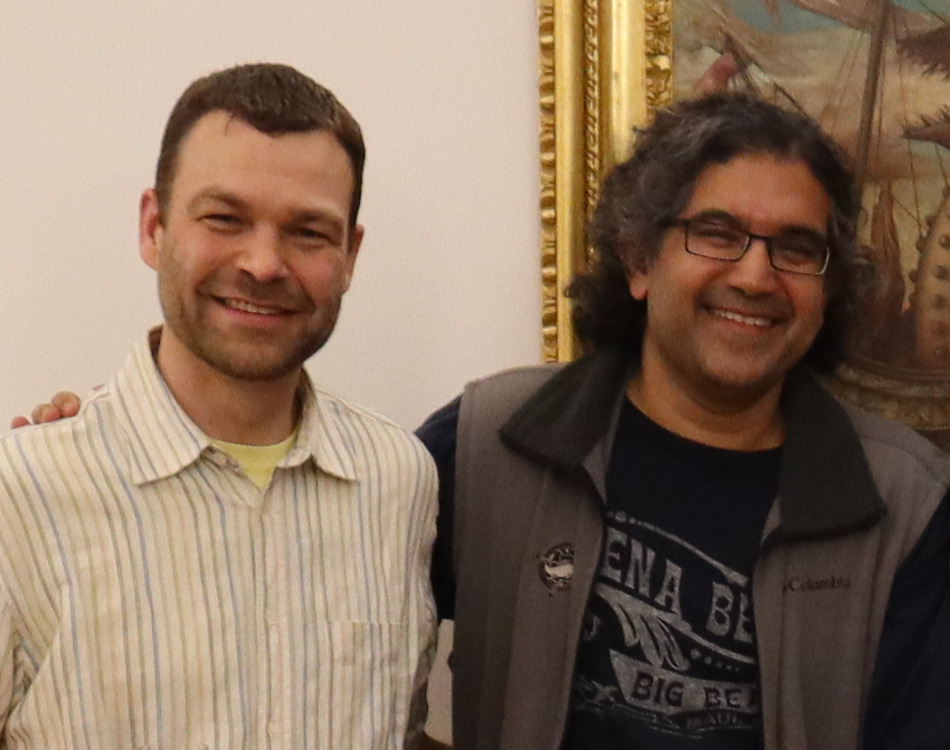
\includegraphics[width=0.35\textwidth]{arni_rishi}
\end{frame}

% ______________________________________________________________________________

\begin{frame}[plain]
  \begin{tikzpicture}[remember picture,overlay]
    \node[at=(current page.center)]
    {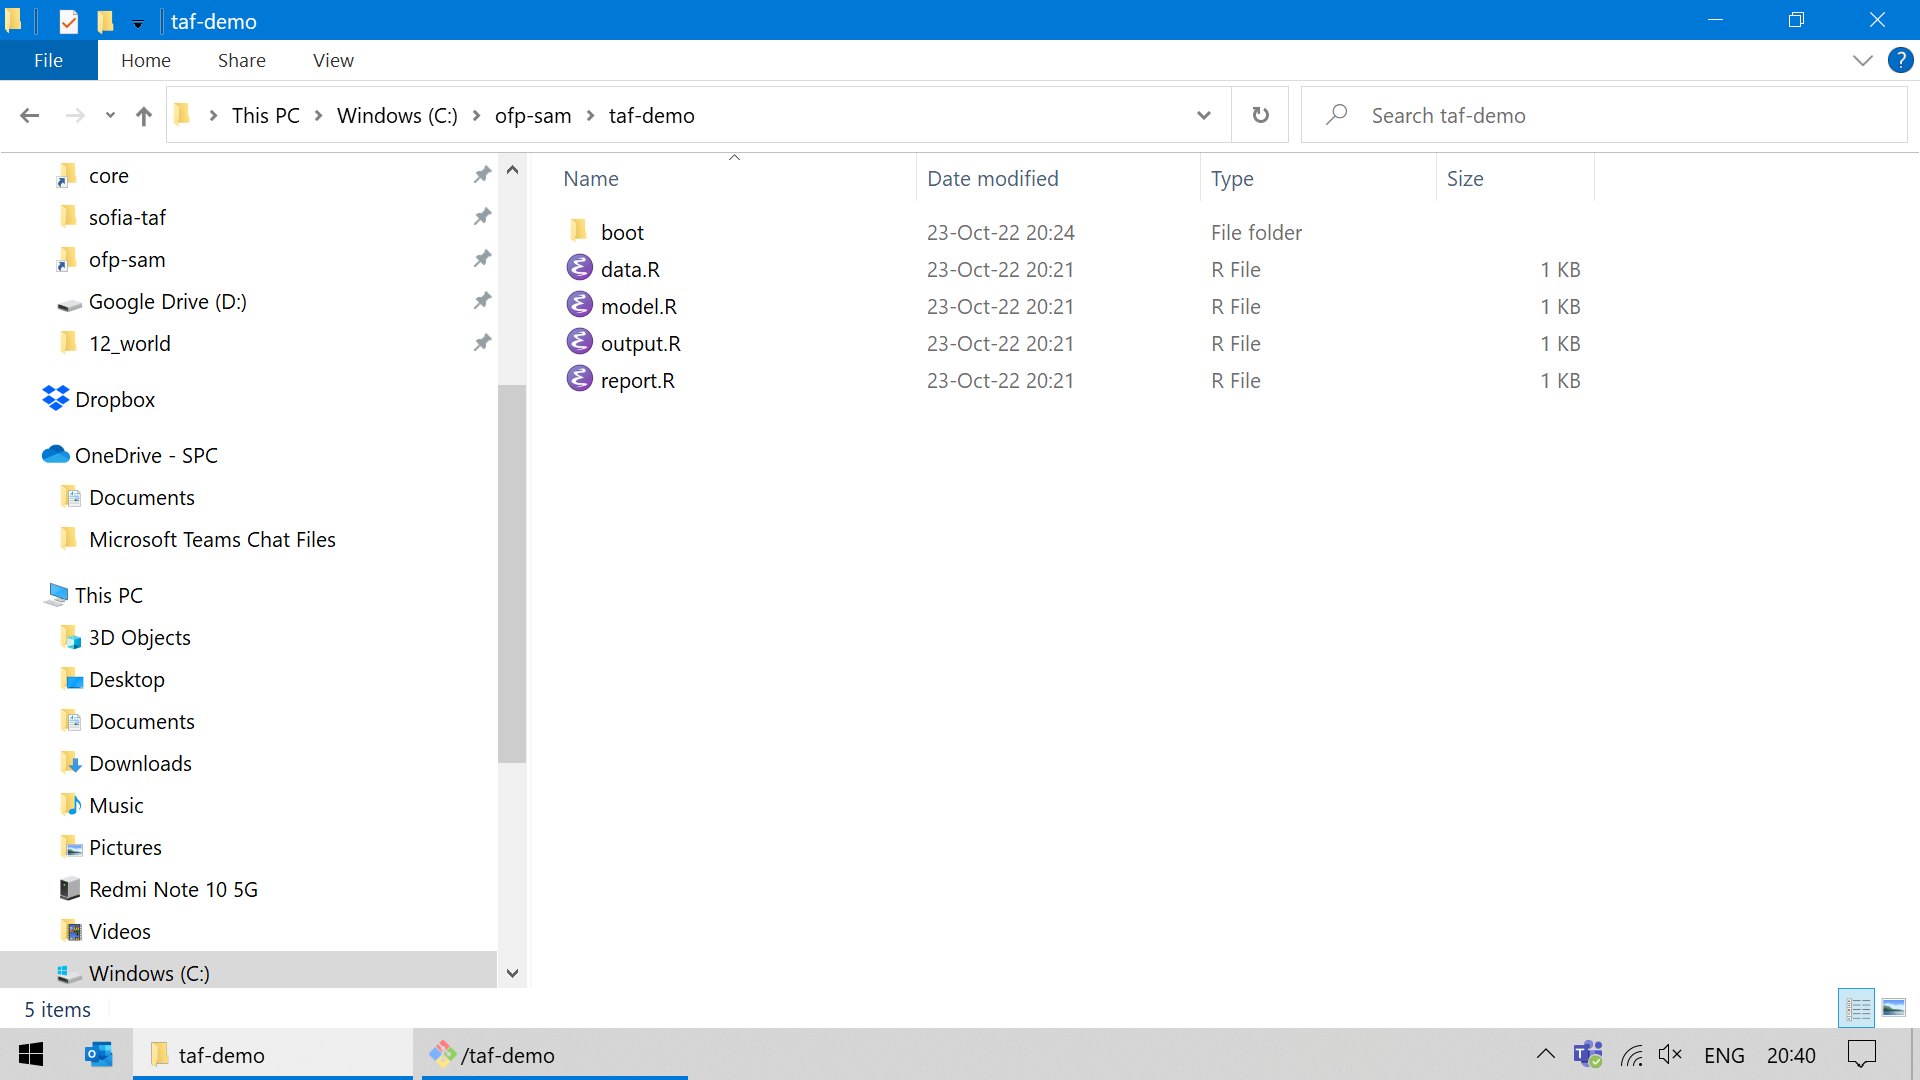
\includegraphics[width=\paperwidth]{taf_explorer_1}};
  \end{tikzpicture}
\end{frame}

% ______________________________________________________________________________

\begin{frame}[plain]
  \begin{tikzpicture}[remember picture,overlay]
    \node[at=(current page.center)]
    {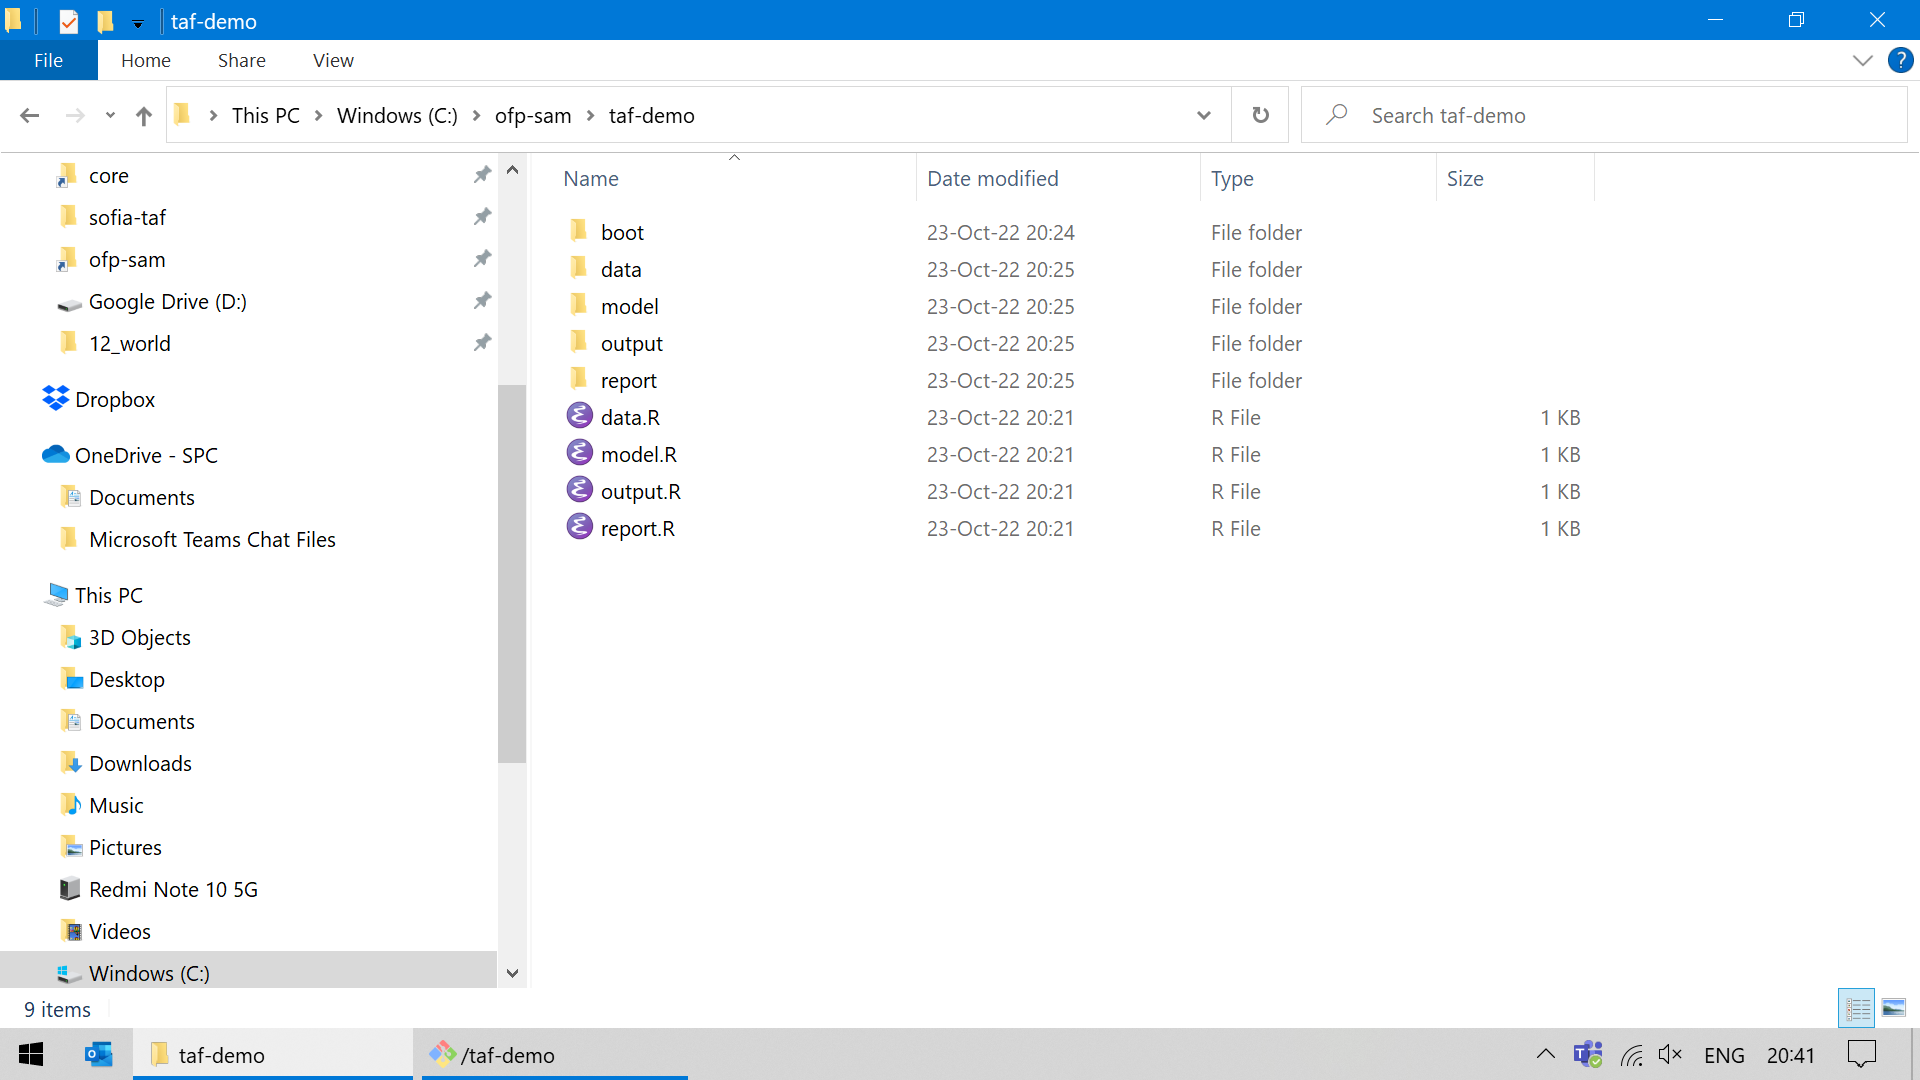
\includegraphics[width=\paperwidth]{taf_explorer_2}};
  \end{tikzpicture}
\end{frame}

% ______________________________________________________________________________

\begin{frame}{SOFIA-TAF}
  \centering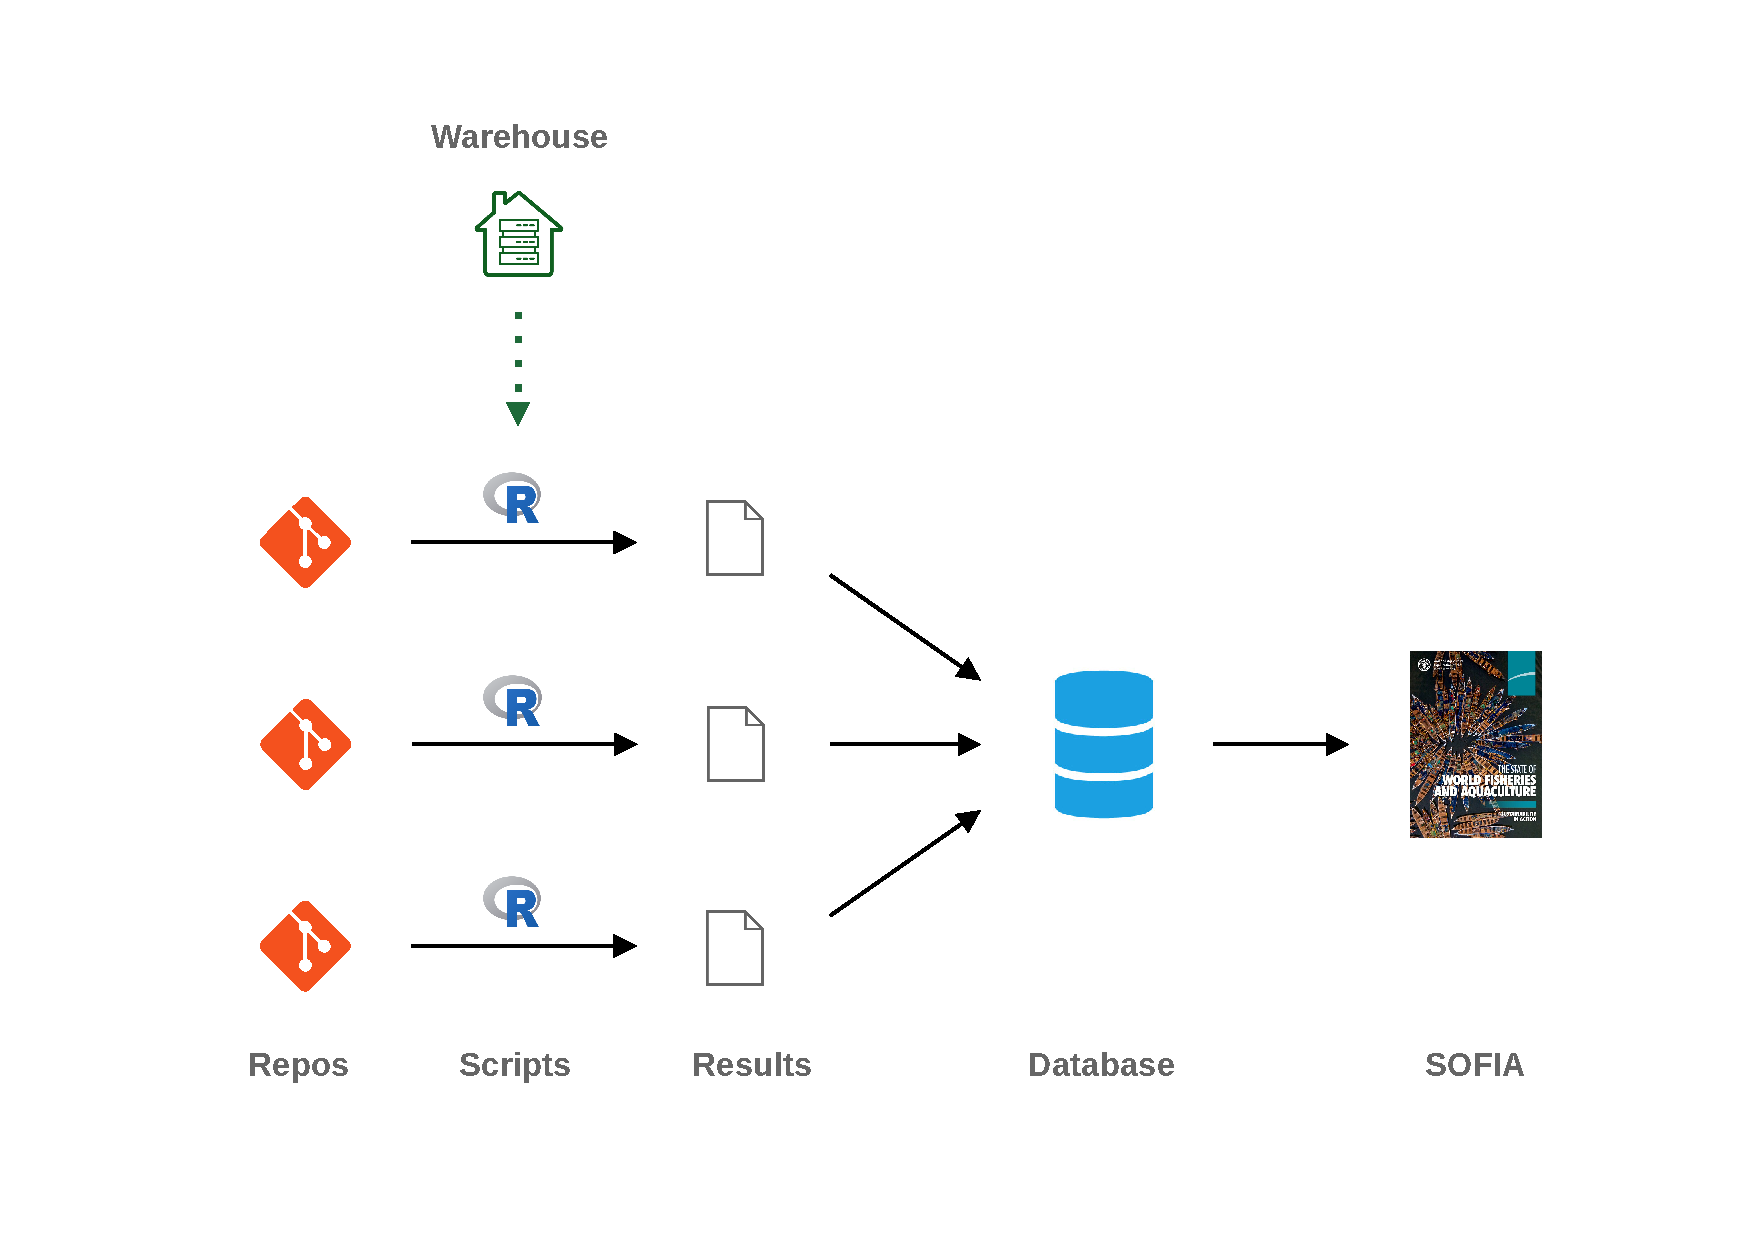
\includegraphics[height=0.7\textheight]{sofia_diagram}
  \vspace{2ex}
\end{frame}

% ______________________________________________________________________________

\begin{frame}{Open Science Infrastructures}
  \textbf{\blue Some examples from fisheries}\\[1ex]
  \begin{tabular}{lll}
    2018 & ICES & ICES-TAF \\[0.5ex]
    2021 & FAO  & GFCM STAR\\[0.5ex]
    2022 & FAO  & SOFIA-TAF\\[0.5ex]
    2023 & SPC  & Assessment Repos\\[5ex]
  \end{tabular}\\
  \textbf{\green\bf General}\\[1ex]
  \begin{tabular}{ll}
    2021 & UN Recommendation on Open Science\\[0.5ex]
    ~    & \arrow adopted by 193 member states, provides principles and
           norms\\[0.5ex]
    2022 & UN Working Group on Open Science Infrastructures\\
  \end{tabular}
\end{frame}

% ______________________________________________________________________________

\begin{frame}{Discussion}
  There are two types of scripts\\[2ex]
  \begin{enumerate}
    \item Script that {\bf runs}\\[0.5ex]
    \comment{relatively short, does one part of the workflow, as reflected by
      its filename\\
      \h{2.5ex}{\gray $\Rightarrow$ to use this script:}
      {\orange run it}}\\[2ex]
    \item Script that is {\bf essentially a notebook}\\[0.5ex]
    \comment{longer, does many parts of the workflow,\\
      \h{2.5ex}not really intended to run completely from start to finish\\
      \h{2.5ex}{\gray $\Rightarrow$ to use this script:}
      {\orange open and run selected blocks of code}}\\[3ex]
  \end{enumerate}
  It's useful to clearly distinguish between these types of scripts (1st and 2nd
  class)\\[0.2ex]
  and consider what is most practical for a given project\\[1ex]
\end{frame}

% ______________________________________________________________________________

\begin{frame}{Discussion}
  \textbf{\green Data preparation} is a large part of the stock assessment
  work\\[2ex]
  \begin{itemize}
    \item[] Indices \comment{survey, cpue}
    \item[] Catch \comment{in tonnes, age composition, size composition}
    \item[] Life history \comment{maturity, growth}
    \item[] Tags \comment{releases, recaptures}
    \item[] etc.\\[3ex]
  \end{itemize}
  The benefits of {\bf scripting the data preparation} as reproducible workflows
  can be\\[0.2ex]
  at least as important and benefitial as scripting the model run\\[2ex]
\end{frame}

% ______________________________________________________________________________

\begin{frame}{Recommendations}
  \textbf{\green Project organization}
  \begin{enumerate}
    \item Organize analyses in GitHub repos, preferably open (at least scripts)
    \item Divide the work into separate scripts of manageable size, with
    descriptive names
    \item Make each script run by itself: read files, do stuff, write files
    \item Consider using a common structure to organize projects\\[3ex]
  \end{enumerate}
  \textbf{\green Within each script}
  \begin{enumerate}
    \item Write the script so it will run on any computer
    \item Avoid using setwd() {~\quad\small\gray use alt-sws in RStudio}
    \item Use relative paths
    \item Use few dependencies {~\quad\small\gray Chuck Norris style}
  \end{enumerate}
\end{frame}

% ______________________________________________________________________________

\begin{frame}{Transparency in Fisheries Management}
  \textdarkgreen{Transparent} = open and reproducible\\[0.4ex]
  \h{14.4ex}as a result, reviewable and traceable\\[6ex]
  A growing question in all fisheries around the world:\\[0.4ex]
  \quad{\bf $\Rightarrow$ Is the management of this stock based on open and
    reproducible science?}\\[6ex]
  {\em If not, which criteria are still missing?}
  \vspace{2ex}
\end{frame}

% ______________________________________________________________________________

\begin{frame}{Overview}
  \begin{itemize}
    \item[] {\bf\darkblue Why} \comment{repeatability, institutional memory,
      reviewability, scientific method,\\
      \h{8.5ex}interregional research, dissemination, collaboration,
      traceability, credibility}\\[3ex]
    \item[] {\bf\darkblue Open} \comment{scripts, data, software}\\[3ex]
    \item[] {\bf\darkblue Reproducible} \comment{standardized sequential R
      scripts, version control}\\[3ex]
    \item[] {\bf\darkblue Infrastructure}
    \comment{2021 UN Recommendation on Open Science, working group,\\
      \h{18.6ex}GitHub, TAF, data management, ICES, FAO, GFCM, SPC}\\[3ex]
    \item[] {\bf\darkblue Recommendations}
    \comment{relative paths, dependencies, 1st and 2nd class scripts,\\
      \h{23.9ex}complete workflow, data preparation, partially open}\\[3ex]
  \end{itemize}
\end{frame}

\end{document}
